\documentclass[a4paper]{article}

\usepackage[czech]{babel} %https://github.com/michal-h21/biblatex-iso690
\usepackage[
   backend=biber      % if we want unicode 
  ,style=iso-numeric % or iso-numeric for numeric citation method          
  ,babel=other        % to support multiple languages in bibliography
  ,sortlocale=cs_CZ   % locale of main language, it is for sorting
  ,bibencoding=UTF8   % this is necessary only if bibliography file is in different encoding than main document
]{biblatex}

\usepackage[utf8]{inputenc}
\usepackage{fancyhdr}
\usepackage{amsmath}
\usepackage{amssymb}
\usepackage[left=2cm,right=2cm,top=2.5cm,bottom=2.5cm]{geometry}
\usepackage{graphicx}
\usepackage{pdfpages}
\usepackage{url}
\usepackage{multirow}

\usepackage{siunitx}
\sisetup{locale = DE, separate-uncertainty = true} %   kdybych chtel +/-

\usepackage{float}
\newfloat{graph}{htbp}{grp}
\floatname{graph}{Graf}
\newfloat{tabulka}{htbp}{tbl}
\floatname{tabulka}{Tabulka}

\renewcommand{\thefootnote}{\roman{footnote}}

\pagestyle{fancy}
\lhead{Praktikum II - (18) Přechodové jevy v RLC obvodu}
\rhead{Vladislav Wohlrath}
\author{Vladislav Wohlrath}

\bibliography{source}

\begin{document}

\begin{titlepage}
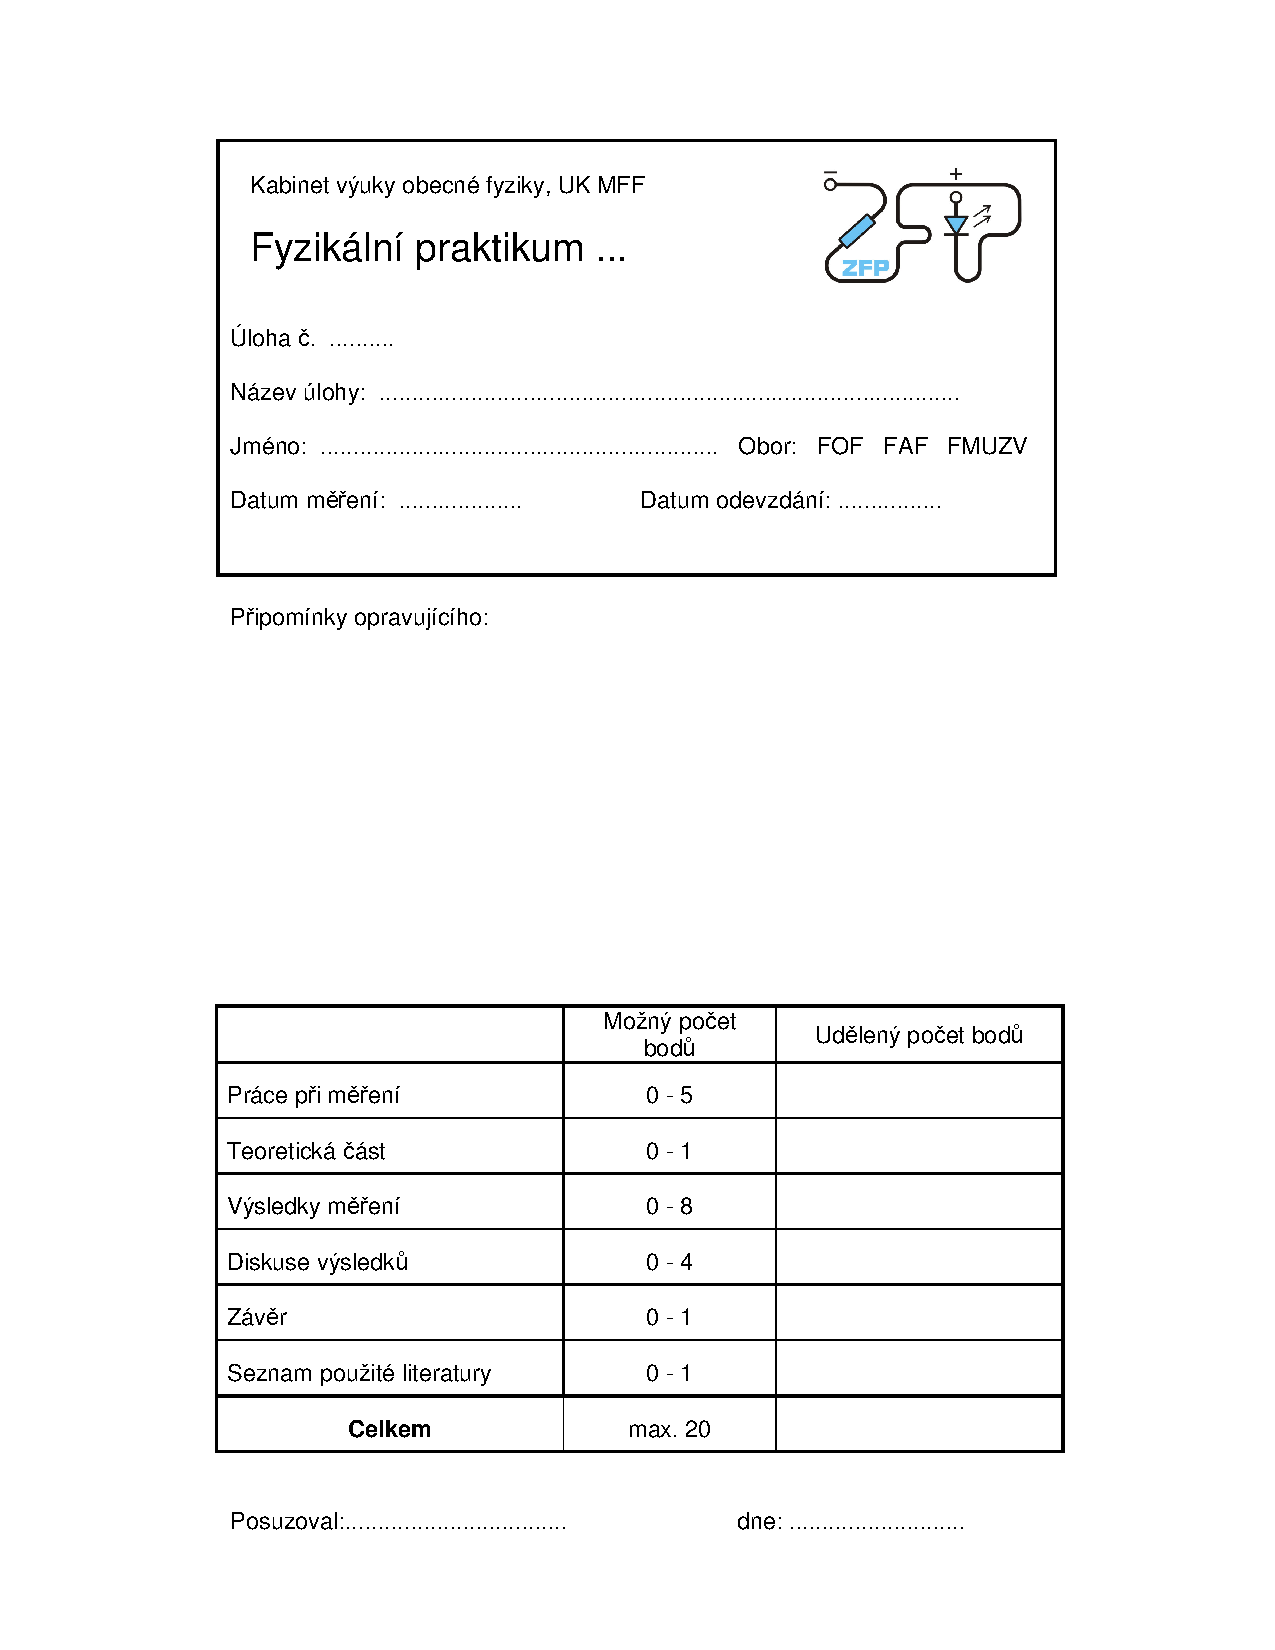
\includepdf[pages={1}]{./graficos/titlelist.pdf}
\end{titlepage}

\section*{Pracovní úkoly}
\begin{enumerate}
\item Sestavte obvod podle obr. 1 (viz studijní text k úloze) a změřte pro obvod v periodickém stavu závislost doby kmitu $T$ na velikosti zařazené kapacity alespoň pro pět hodnot z intervalu ($C$=\num{0.1}--\SI{10}{\micro\farad}, $R$ = \SI{20}{\ohm}). Výsledky měření zpracujte graficky a vyhodnoťte velikost indukčnosti $L$ zařazené v obvodu.
\item Stanovte hodnoty aperiodizačních odporů pro pět hodnot kapacit zařazeného kondenzátoru. I v tomto případě stanovte velikost indukčnosti $L$.
\item Změřte závislost relaxační doby seriového obvodu RC podle obr. 2 (viz. studnijní text k úloze) na velikosti odporu a na velikosti kapacity v obvodu. Výsledky měření zpracujte graficky a porovnejte s teoretickými.
\end{enumerate}

%Teoretická část
\section*{Teoretická část}

%Výsledky měření
\section*{Výsledky měření}

%Diskuze výsledků
\section*{Diskuze}
Měření periody i aperiodizačních odporů jsme prováděli s touž cívkou, takže pokud by byla obě měření správná, měly by se hodnoty $L_1=\SI{0.52(5)}{\henry}$ a $L_2=\SI{0.34(2)}{\henry}$ shodovat, což v našem případě platí jen řádově.


Měření aperiodizačních odporů bylo zatíženo velkou systematickou chybou, protože záleželo na tom, jestli daný průběh vyhodnotím jako periodický či aperiodický.
Pokud je hodnota $L_1$ správná, znamenalo by to, že je buď měření zatíženo nějakou jinou neznámou systematickou chybou, nebo jsme hodnoty $R_{ap}$ určili přibližně \num{1.2} krát menší.
Signál byl zatížen nezanedbatelným šumem, takže je možné, že druhý kmit již byl pod hranicí šumu, a proto nebylo možné ho pozorovat a došlo tak k mylnému označení průběhu za aperiodický.
Z těchto důvodů považuji hodnotu $L_1$ za přesnější.

Při fitování průběhu proudu RC obvodem se u všech měření stalo to, že hodnoty na kraji měřeného časového intervalu ležely znatelně pod proloženou křivkou, zatímco hodnoty ve středu ležely nad ní.
Průběh tedy nebyl přesně exponenciální.
Nicméně naměřené relaxační doby se velmi dobře shodují s teoretickými, žádná se neliší o více než \SI{5}{\percent}.

%Závěr
\section*{Závěr}


\printbibliography[title={Seznam použité literatury}]

\end{document}